

%\begin{titlepage}
	\thispagestyle{empty}
	\addcontentsline{toc}{chapter}{الغلاف}
	
	\newfontfamily\coverfont[Script = Arabic, Ligatures = TeX, SizeFeatures={Size=16}]{Traditional Arabic}
	\newfontfamily\authorsfont[Script = Arabic, Ligatures = TeX, SizeFeatures={Size=18}]{Traditional Arabic}
	
	{
		\begin{wrapfigure}{l}{0.25\textwidth}
			\hfill
			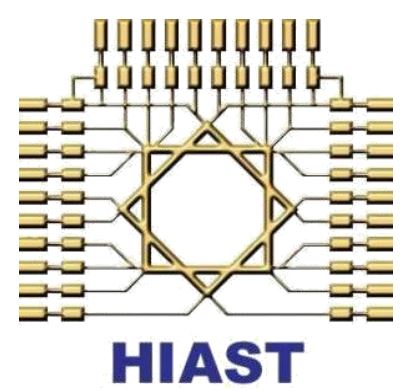
\includegraphics[width=0.9\linewidth]{images/HIAST_logo.JPG}
		\end{wrapfigure}
			
		\coverfont
		\begin{spacing}{1.8}
			\ \\
			الجمهورية العربية السورية \\
			المعهد العالي للعلوم التطبيقية والتكنولوجيا \\
			قسم المعلوميات \\
			العام الدراسي 2017/2018  \\
		\end{spacing}
	}
	
	
	\vspace{2cm}
	\begin{center}
		{
			\Huge
%			تقييم جودة نصوص اللغة الانكليزية

%			بناء مُصنّف لتقييم سهولة قراءة نصوص اللغة الانكليزية 
%			وفق عدّة مستويات باستخدام تعلم الآلة

			نظام خبير لتقييم مقروئية نصوص اللغة الانكليزية وفق عدّة مستويات
			\\[2.5mm]
			\Large
			مشروع السنة الرابعة
		}
	
		\vspace{3cm}
		\begin{doublespace}
			إعداد \\
			{
				\authorsfont
				فاروق حجابو \\[7mm]
			}
			إشراف \\[3mm]
			{
				\authorsfont
				د. غيداء ربداوي
				\hspace{2.5cm}
				م. رياض سنبل
			}
		\end{doublespace}
	\end{center}
		
	\vfill
	\centerline{2 أيلول 2018}
	
%\end{titlepage}


